\documentclass[10pt,a4paper]{article}
\usepackage[utf8]{inputenc}
\usepackage{amsmath}
\usepackage{amsfonts}
\usepackage{amssymb}
\usepackage{graphicx}
\usepackage[left=2cm,right=2cm,top=2cm,bottom=2cm]{geometry}

\title{TyPy: A Python Bytecode Interpreter for the Browser}
\author{Puja Mishra, Kate Silverstein}
\date{27 October 2014}

\begin{document}
\maketitle
\section{Understanding the Requirements}

The goal of this project is to implement a Python bytecode interpreter which is engine dependent and also can be hosted on a variety of browsers. So the high level picture of how we have implemented is shown below.

\begin{figure}[ht!]
\center
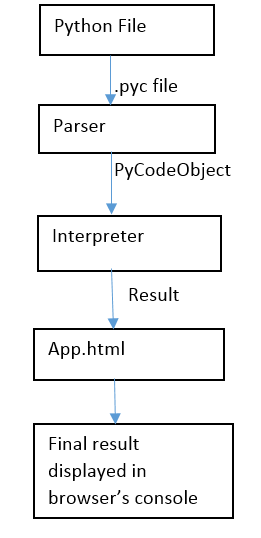
\includegraphics[scale=1]{../Report/UnderstandingTheReq.png} 

\end{figure}

\section{Design Approach}

The input to the system is the python program written by the user and compiled using "compileall" module. This *.pyc file is uploaded when the user opens application, this file is passed to the parser where parser parses the bytecodes and generates a PyCodeObject to the the interpreter (which here is a stack based interpreter) , which interprets it and gives the result on the browser's console.



\subsection{Parser}
% general structure of parser taken from UnPyc

\subsubsection{Structure of a Python Bytecode File}
The bytecode is an attribute of the code object and is found in cocode attribute of the code object and contains instructions for the interpreter. Bytecode is nothing but a series of bytes.The interpreter will loop through each byte, look up what it should do for each one, and then do that thing. Using the dis module we can disassemble the bytecode.


% \subsection{Character Encoding Considerations} (if there's time?)

\subsection{Interpreter Design}
We borrowed the general structure of our interpreter from byterun and adopted it to our design. It is a stack based interpreter where the bytecodes are parsed and put on the stack and interpreted by manipulating the items on the stack.

% general structure of interpreter taken from byterun 

\subsubsection{Stack-Based Interpreters} 
% talk about these vs. alternatives? (CPython is stack-based) (vs register-based? PyPy?)

\subsubsection{Implementation for TyPy}
% ks

\subsection{Other Design Considerations}
\subsubsection{Client-Side vs. Server-Side Javascript}
% have to store files in browser local storage
% have to use BrowserFS instead Node.js
% have compile using AMD module instead of commonjs module (why did this matter? what are differences?)
% have to use RequireJS to import

\subsection{Test Suite}
% CORS request to test server (Express)

\section{Implementation Results}
\subsection{Supported Functionality}
The interpreter we have implemented can interpret simple "if" statements, for and while loops, basic list creation and indexing, basic dictionary creation and queries, basic math operations.
% sample output from browser console

% \subsection{Runtime and Efficiency} %(if there's time)
% how long does it take to run e.g. sorting a list for a huge list?

\section{Future Work}
As an extension of the project we can add more functionality which can help to interpret complex functions written in python.

\section{Conclusion}
Working on this project has been a very good and learning  experience. The system implemented by us is a simple interpreter which can interpret basic functionality written in python.

\section{References} % generate bibliography?
% UnPyc
% byterun
% CPython
% BrowserFS

\begin{thebibliography}{9}

\bibitem{byterun}
  Ned Batchelder,
  \emph{byterun }.
  https://github.com/nedbat/byterun


\end{thebibliography}




\end{document}


